\begin{theo}[Elektrische flux]{Elektrische flux}

    % Het concept van \textbf{elektrische flux} zal heel interessant blijken, vooral omdat dit ons een nieuwe methode geeft om elektrisch velden te berekenen. 
    
    De elektrische flux doorheen een oppervlak is de oppervlakte-integraal van de elektrische veldsterkte over dat oppervlak. Laten we eerst kijken naar, zoals vaker, het makkelijker geval, namelijk wanneer we spreken over een uniform elektrisch veld:
    
    \begin{equation*}
        \Phi_E = \Vec{E}\cdot\Vec{A}
    \end{equation*}
    
    \noindent Als we spreken over een niet-uniform veld, dan spreken we eigenlijk over infinitesimale uniforme velden. De formule wordt dus:
    \begin{equation*}
        \Phi_E = \oint \Vec{E}\cdot d\Vec{A}
    \end{equation*}
    
    \noindent De nettoflux $ \Phi_e $ is recht evenredig met netto aantal veldlijnen dat het oppervlakte verlaat.
    
        \begin{center}
            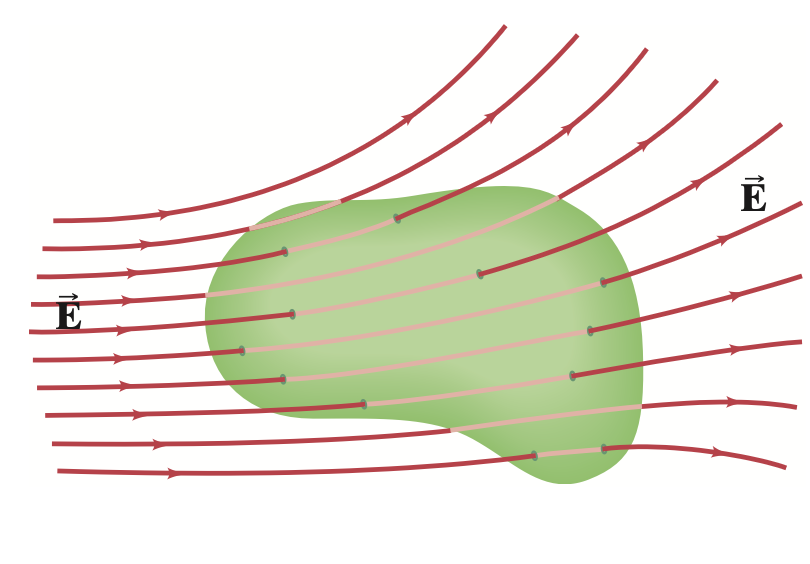
\includegraphics[scale = 0.35]{Images/Elektriciteit/OppervlakteGeenLading.png}
        \end{center}
    % Sinds er een verband is tussen elektrisch veld en gravitatieveld, kunnen we ook praten over gravitationele flux bij dynamica.
\end{theo}

\begin{lem}[Gauss]{Gauss}

    De wet van Gauss luidt: de nettoflux door een willekeurig \textbf{gesloten} oppervlak dat een lading $ q $ omsluit, is steeds gelijk aan $ \tfrac{q_{in}}{\epsilon_0} $. In formulevorm:
    
    \begin{equation*}
        \Phi_E = \oint \Vec{E}\cdot d\Vec{A} = \dfrac{q_{in}}{\epsilon_0}
    \end{equation*}
    
    \noindent Hieruit volgt dus dat de nettoflux door een willekeurig gesloten oppervlak dat geen lading omsluit, is steeds gelijk aan 0. 
    % Dit kunnen we intuitief ook makkelijk begrijpen: als er een lading zou zijn, dan zouden de binnenkomende en buitengaande veldlijnen niet meer een gelijk aantal zijn en is dus de nettoflux niet nul.
\end{lem}

% \begin{app}[Wet van Gauss bij meerdere elektrische velden]{Wet van Gauss bij meerdere elektrische velden}
% We kunnen natuurlijk de formule van hierboven ook gebruiken als er meerdere elektrische velden aanwezig zijn. Dit wordt dan door de wet van de superpositie:

% \begin{equation*}
%     \Phi_e = \oint \Vec{E}_{tot}\cdot d\Vec{A} = \oint (\sum_i \Vec{E}_i) \cdot d\Vec{A}  = \dfrac{q_{in}}{\epsilon_0}
% \end{equation*}

% \end{app}

% \begin{app}[Wet van Coulomb vs wet van Gauss]{Wet van Coulomb vs wet van Gauss}
%     \begin{center}
%         \def\arraystretch{2.5}
%         \begin{tabular}{c|c}
%             wet van Coulomb & wet van Gauss \\ \hline
%             $ E = k\dfrac{Q}{r^2} $ & $ \oint \Vec{E}\cdot d\Vec{A} = 4\pi kQ$ \\ 
%             $ E = \dfrac{1}{4\pi\epsilon_0}\dfrac{Q}{r^2} $ & $ \oint \Vec{E}\cdot d\Vec{A} = \dfrac{Q_{in}}{\epsilon_0} $
%         \end{tabular}
%     \end{center}
% \end{app}

% \begin{prf}[Formeel bewijs van de wet van Gauss]{Formeel bewijs van de wet van Gauss}

%     \begin{itemize}
%         \item{Lading \emph{binnen} gesloten oppervlak}
            

%             \begin{center}
%                 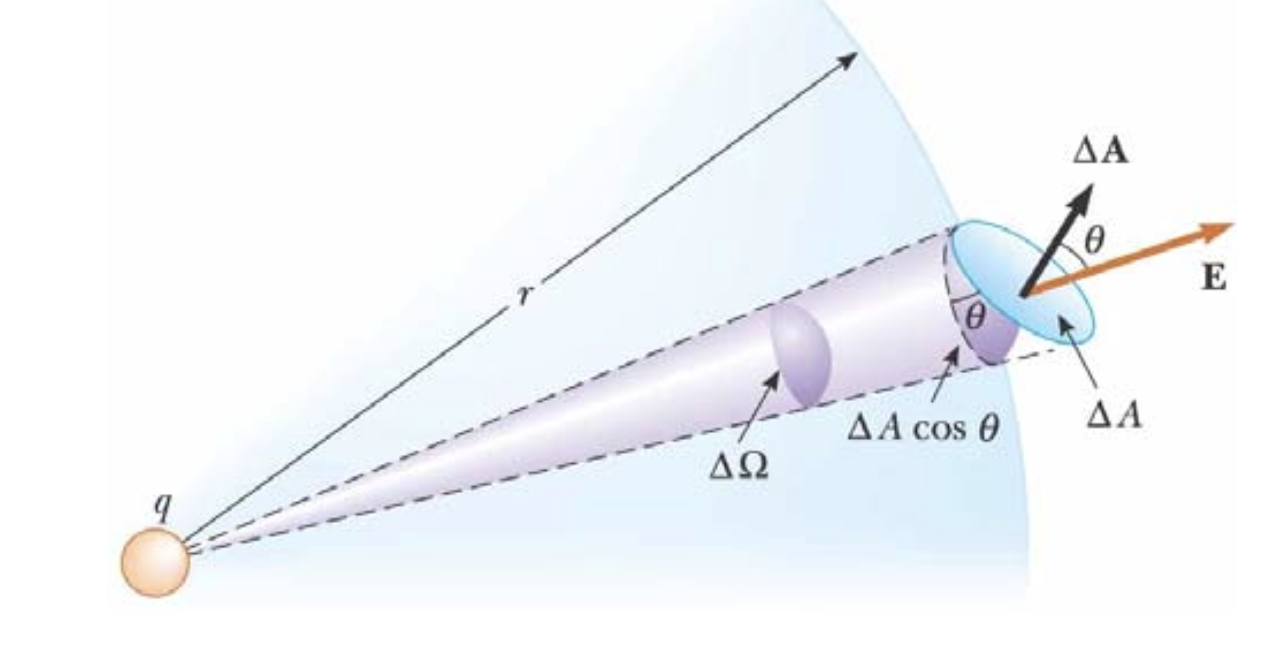
\includegraphics[scale = 0.3]{Images/Elektriciteit/Ruimtehoek.png}
%             \end{center}
        
%         \item{Lading \emph{buiten} gesloten oppervlak}
        
%             \begin{minipage}{.48\textwidth}
%             \end{minipage} 
%             \begin{minipage}{.48\textwidth}
%             \end{minipage}
    
%     \end{itemize}
% \end{prf}

% \begin{pro}[Eigenschappen van geleiders in elektrostatisch evenwicht]{Geleiders in elektrostatisch evenwicht}

%     \begin{minipage}{.55\textwidth}
%         \begin{itemize}
%             \item Elektrisch veld in de geleider is nul
%             \item De lading van een geïsoleerde geleider bevindt zich aan het oppervlak
%             \item Elektrisch veld net buiten de geleider:
%             \begin{itemize}
%                 \item $ E \perp A $
%                 \item $ E = \dfrac{\sigma}{\epsilon_0} $, want: \\
%                         $ \Phi_e = \oint \Vec{E}\cdot d\Vec{A} = EA = \dfrac{Q_{in}}{\epsilon_0} = \dfrac{\sigma A}{\epsilon_0} \Rightarrow E = \dfrac{\sigma}{\epsilon_0}$
%             \end{itemize}
%             \item Oppervlakteladingsdichtheid is grootst bij grootste oppervlaktekromming
%         \end{itemize}
%     \end{minipage} 
%     \begin{minipage}{.41\textwidth}
%         \centering
%         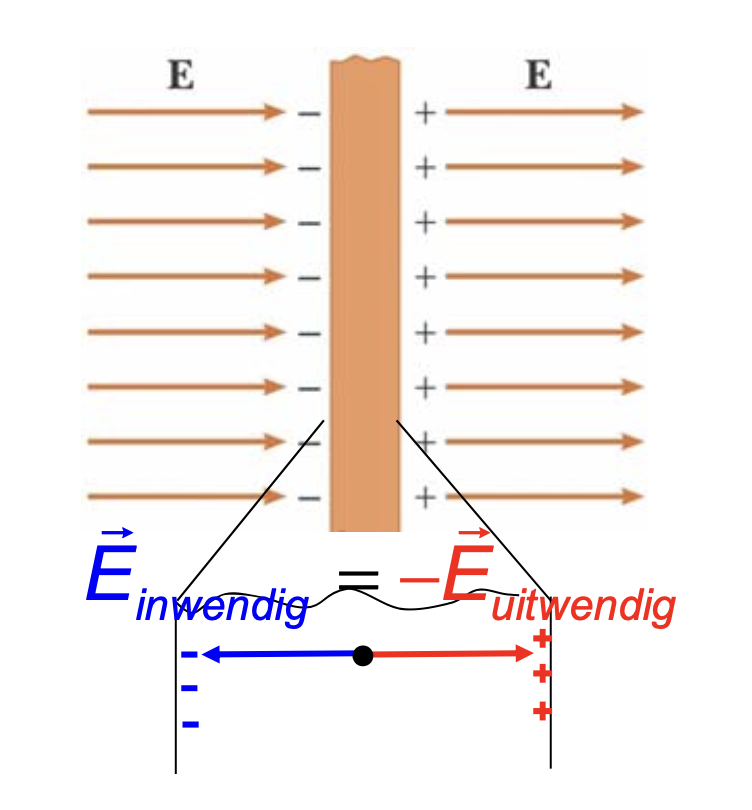
\includegraphics[scale = 0.4]{Images/Elektriciteit/Elektrisch veld in een geleider.png}
%     \end{minipage}

% \end{pro}


